\documentclass[twocolumn, a4paper, 12pt]{article}
\usepackage{graphicx}
\usepackage{amsmath}
\begin{document}
\title{Exponential-function}
\author{Victor Rueskov Christiansen}
\maketitle

\begin{abstract}
The exponential function is a very commonly used function in all areas of science.

\end{abstract}

\section{Introduction}
The natural exponential function, often refered to as simply the exponential function, is a specialixation of the general exponential function with euler's number as the root number. It is defined as
\begin{equation}\label{eq:def}
	\mathrm{exp}(x) = e^x,
\end{equation}
where $e$ is euler's number, approximately $e \approx 2.718...$. The useful property of the exponential function is, that is its own derivative. That is $\partial e^x = e^x$. It is clear from this relation that it is also its own antiderivative.
A more formal definition of the exponential function than eq. ~ (\ref{eq:def}) is the power series of the exponential function
\begin{equation} \label{eq:pow}
	\mathrm{exp}(x) = \sum_k \frac{x^k}{k!} = 1 + x + \frac{x^2}{2} + \dots
\end{equation}
In figure \ref{fig:exp} the exponential function is plotted along with some tabulated values.

\begin{figure}[h]\label{fig:exp}
	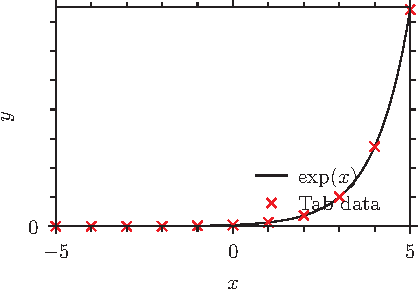
\includegraphics{exp_pyx.pdf}
\end{figure}

\section{Implementation}
Figure \ref{fig:exp} was created using a c-sharp implementation, where the exponential function was defined as a power series like in eq. (\ref{eq:pow}). However for $x > 1/8$, the implementation returned $(\mathrm{exp}(x/2))^2$. In this way, the exponential function is evaluated for smaller and smaller $x$, until $x < 1/8$ at which point it is evaluated as a power series. This works for 2 reasons:
\begin{enumerate}
	\item The power series is a better approximation for small $x$. This is way it is only evaluated for $x<1/8$.
	\item The expression $(\mathrm{exp}(x/2))^2 = \mathrm{exp}(2\cdot x/2) = \mathrm{exp}(x)$.
\end{enumerate}
Using these two properties, it is clear why for large $x$, it is better to calculate the exponential of a smaller value and then using the second property to scale the value up again.

\section{Test}
This method works well in practice as can be seen in figure \ref{fig:exp}. The tabulated values lies on the graph of the exponential function, and thus the implementation actually returns good values (at least for $x$ between -5 and 5 as is plotted here.

\end{document}
